\newpage
\section{Discussion}
\noindent The skateboard trajectories are all very similar to an actual ollie. Without any motion cues, the optimizer is able to replicate the ollie motion, with almost all phenomena seen in \ref{f_olliesteps}. The optimizer shows that the human first jumps, then slams the skateboard to the ground, slides the front foot over the deck to drag it up and level it out and catches the skateboard with the back foot at the highest point. This is very close to reality. The human replicates the counter movement jump with a very similar force graph if figures \ref{f_notail} and \ref{f_GRF} are compared. Also the impact energy is similar to the impulse found in figure \ref{f_GRF}. The impulse from the GRF is roughly 5 [J], which is of the same order of magnitude as the found impact losses in figures \ref{f_nopar}, \ref{f_singlepar}, and \ref{f_multipar}.
A single mass point with two free floating feet controlled by forces and feet location with kinematic constraints are able to simulate the motion and output of a human jumper. 
Nine out of eleven optimal skateboard geometries found higher ollies compared to the popsicle stick skateboard. None of these solutions is proven a global optimum, but the improvement to the base skateboard is something that performs better. Skateboard builders should try to implement found geometries and test empirically if they will improve ollie height. These geometries could be a tool to alter existing skateboards and let athletes jump higher. The kinetic and kinematic constraints are of a specific person. The geometries might be dependent on the human capabilities. Empirical testing is necessary to prove that this finding is true in a real life ollie. I successfully solved the ollie optimization problem with a geometry optimization. Compared to others Shield et al. \cite{shield_contact-implicit_2022} who solved an optimization problem for the ollie, my optimization was faster (3 min vs. 43 min), included an geometry optimization, and had a more difficult objective function. The Shield optimization was was set at a fixed ollie height and needed motion tracking to solve optimally. My optimization had a null seed initial guess, with an objective function that maximized ollie height. Such objective functions are generally hard to solve, for example in \cite{nitschke_efficient_2020} first tracking data needs to be implemented to solve a more difficult objective. Step by step less data can be used to solve for an more difficult objective. In the case of this paper, the solution is found without any tracking data and a difficult objective function. 
\subsection{Findings}
\noindent\textbf{Lower inertia and skateboard mass is beneficial for ollie height.} In all parameter optimizations that improved ollie height compared to the base, a reduction in mass and inertia is found. This is logical when looking at the Newton-Euler equations $Force = Mass \times Acceleration$ and $Moment = inertia \times angular acceleration$ The lower the mass, the higher the acceleration the easier the skateboard can go up. With lower inertia the skateboard rotates more easily which minimizes the amount of force needed with the leveling out of the skateboard during upward motion. If that amount of force is lower, the skateboard is pushed down less, which results in a higher ollie. 
   % IF THESE SOLUTIONS ARE GLOBAL OPTIMA
   
\noindent\textbf{Popsicle stick skateboard is close to optimum and slight changes due to preference will not influence the ollie height too much.} As seen with the single parameter optimizations the increase in ollie height was minimal (0.05-0.023 [m]). Only when multiple parameters are changed the ollie height increased significantly (0.074-0.106 [m]), but the shapes are completely different from a popsicle stick skateboard. If skateboarding will keep the popsicle stick skateboard as standard due to the fact that other tricks need to be performed other than the ollie, not much can be changed to the skateboard to optimize it. If the skateboard will change completely, the ollie height could be improved. The wheelbase effects the ollie height the most of all single parameter optimizations, which could be a promising outcome since it does not influence the board shape which is crucial for other tricks. 

\noindent\textbf{Extremely fast optimal solution is found and easy convergence.} The ollie optimization by Shield et al. \cite{shield_contact-implicit_2022} was without a parameter optimization of the skateboard. This optimization took about 43 minutes to solve, and accurate initial guesses were needed for feasible results. The full code presented by me took under 3 minutes to solve. This includes derivation of the Equations of Motion and all constraints, the time to transcribe the problem and to solve in IPOPT. This was all done without initial guesses and solved optimally.


\noindent\textbf{Optimal back foot position is influenced by the leg characteristics of the performer.} In all optimizations the back foot is sitting in the pocket of the skateboard. For example imagine a simple lever system with a fixed force magnitude perpendicular to the lever with distance x from the rotation point. The higher x, the more torque can be generated, but the greater the distance ($s$) the force will travel. In other words $P = F \delta s = F v $. With a fixed power there has to be a trade of between force and velocity. In this case velocity of the back foot is minimized by setting the back foot in the pocket. According to a jumping theory by Morin an Samozino \cite{morin_biomechanics_2018}, jumping output is bound by a force velocity curve, where maximum force can be exerted at zero speed and maximum velocity at zero force. Athletes have different force velocity profiles where one prefers high force output over high velocity and vice versa. The controller preferred the force profile by minimizing the back foot velocity. This finding leads to the conclusion that athletes with different leg profiles should place their feet differently during the ollie. Where a force-profile should set the back foot in the pocket and a velocity-profile on the tip of the skateboard. See figure \ref{FVcurve} for force and velocity oriented human leg output.

\begin{figure}
    \centering
    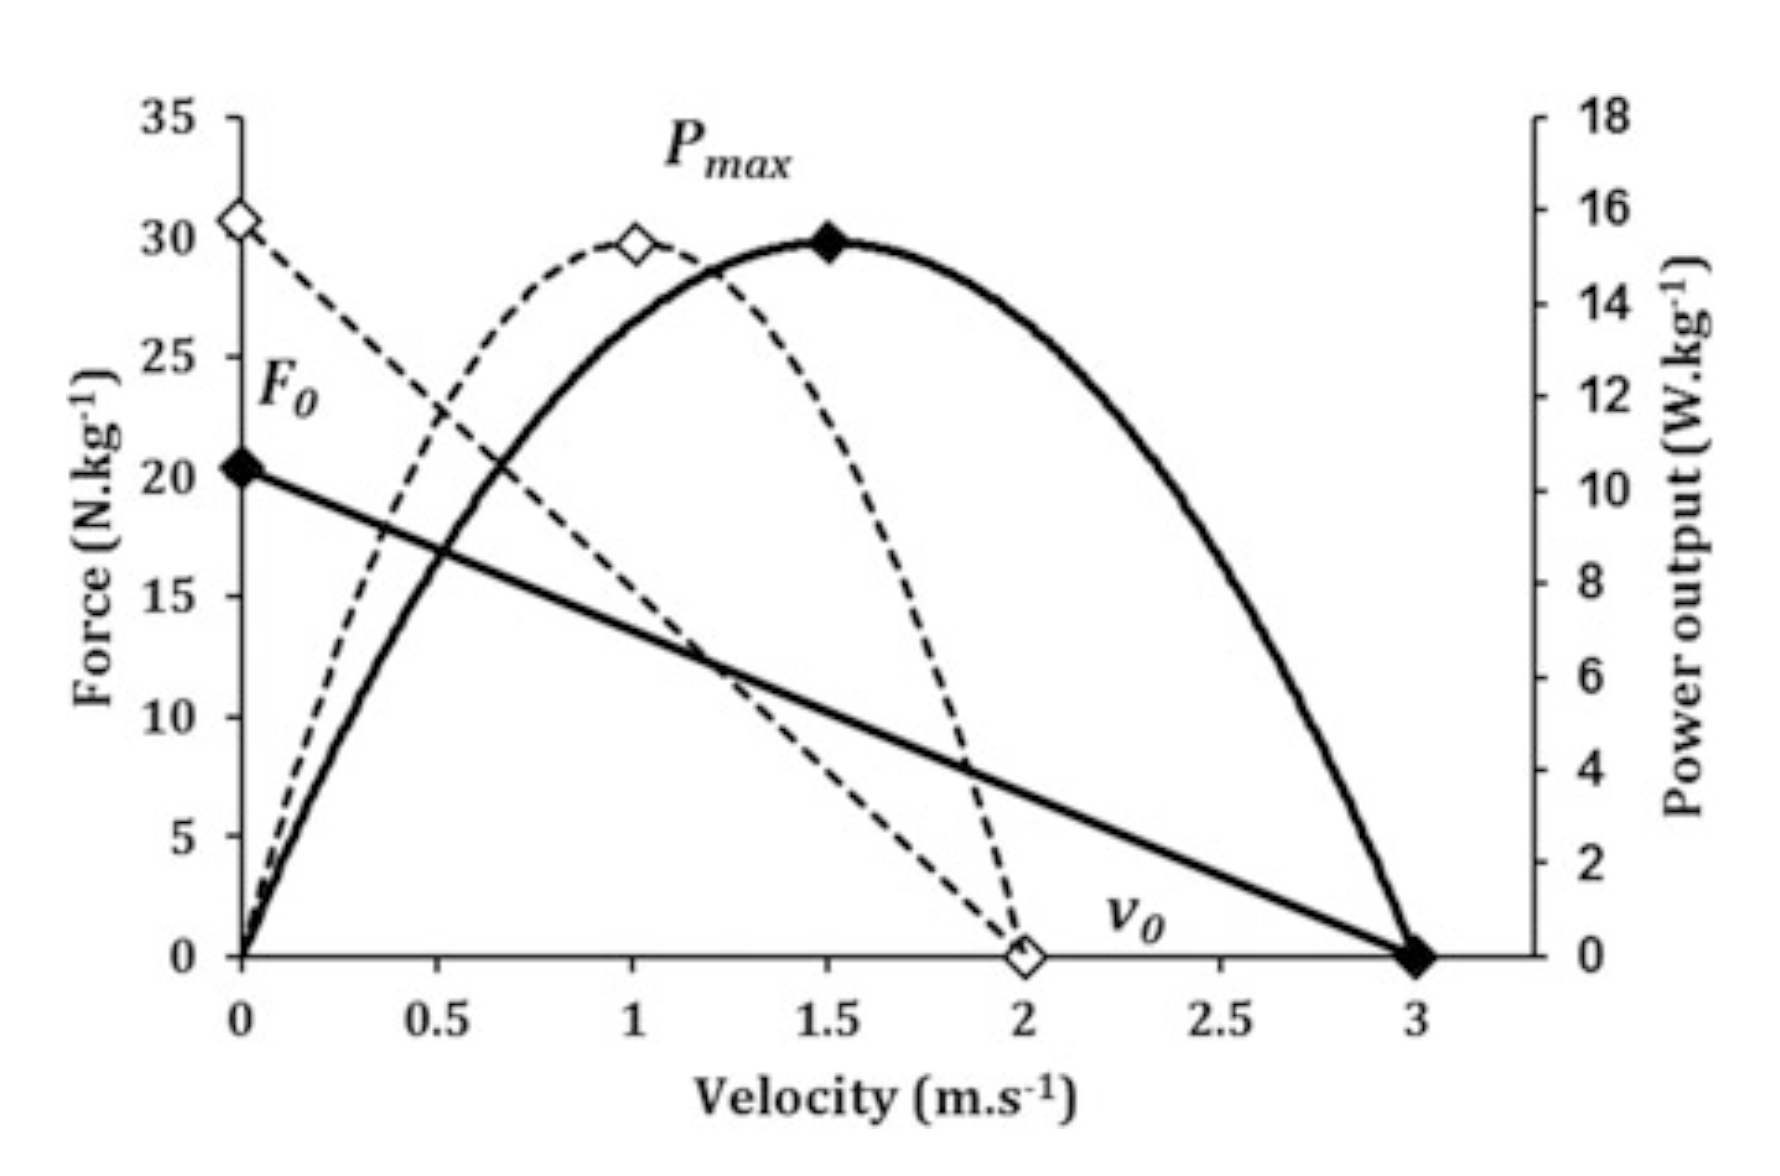
\includegraphics[width = 0.4\textwidth]{figure/Schermafbeelding 2022-11-21 om 16.08.08.png}
    \caption[F-v curve]{Theory on human leg output during jumping. When increasing the load, the maximal force and velocity stay on the line. The dotted line shows a more force oriented human, whereas the other shows a more velocity preferred human jumper. Both have the same maximal power output}
    \label{FVcurve}
\end{figure}

\noindent\textbf{Highly adoptable model.} The presented model can be adjusted to the kinetic and kinematic bounds with little effort. The possibility to optimize a skateboard for a specific athlete is not hard to implement but the kinetic data should be present. Also preference bounds such as width are easily implemented.

\noindent\textbf{Inertia and mass model inertia and mass model for a skateboard is presented that can estimate the dynamic board behaviour in 2D}. The model should be verified with multiple skateboard geometries.

\noindent\textbf{Well represented kinetics.} All results show high similarities between the force profiles of the counter movement jump seen in figure \ref{f_cmj}. The sum of the human kinetics are well bound and show constant results. Even though it is a highly simplified model, the output of the forces is very similar to the output of a CMJ. The point mass model is insightful for the dynamics and is able to show valid results. \\

\noindent\textbf{A fundamentally different simplified contact implicit optimization is made.} The relaxed formulation by Patel et al. \cite{patel_contact-implicit_2019} has been simplified by restating the contact definition. Static and dynamic friction is achieved with the ability to have contact implicit events.

%This book has a chapter about practical implementations on estimating the ballistic performance. The theory says the legs can only produce a certain force at a certain speed, which gives a straight line between the maximum velocity and maximum speed (see fig. \ref{fv}). F0 represents the maximal external force lower limbs could produce during a theoretical extension movement at null velocity. v0 corresponds to the maximal velocity at which lower limbs could extend  under zero load. The values for F0 and v0 are taken from a theoretical optimum for jumping under an angle at 90 degrees with a jump height of 50 [cm] and a maximum power output of 40 [W/kg] at degrees giving: $F0 = 3200 $ and $v0 = 4$. \

% \begin{figure}
%     \centering
%     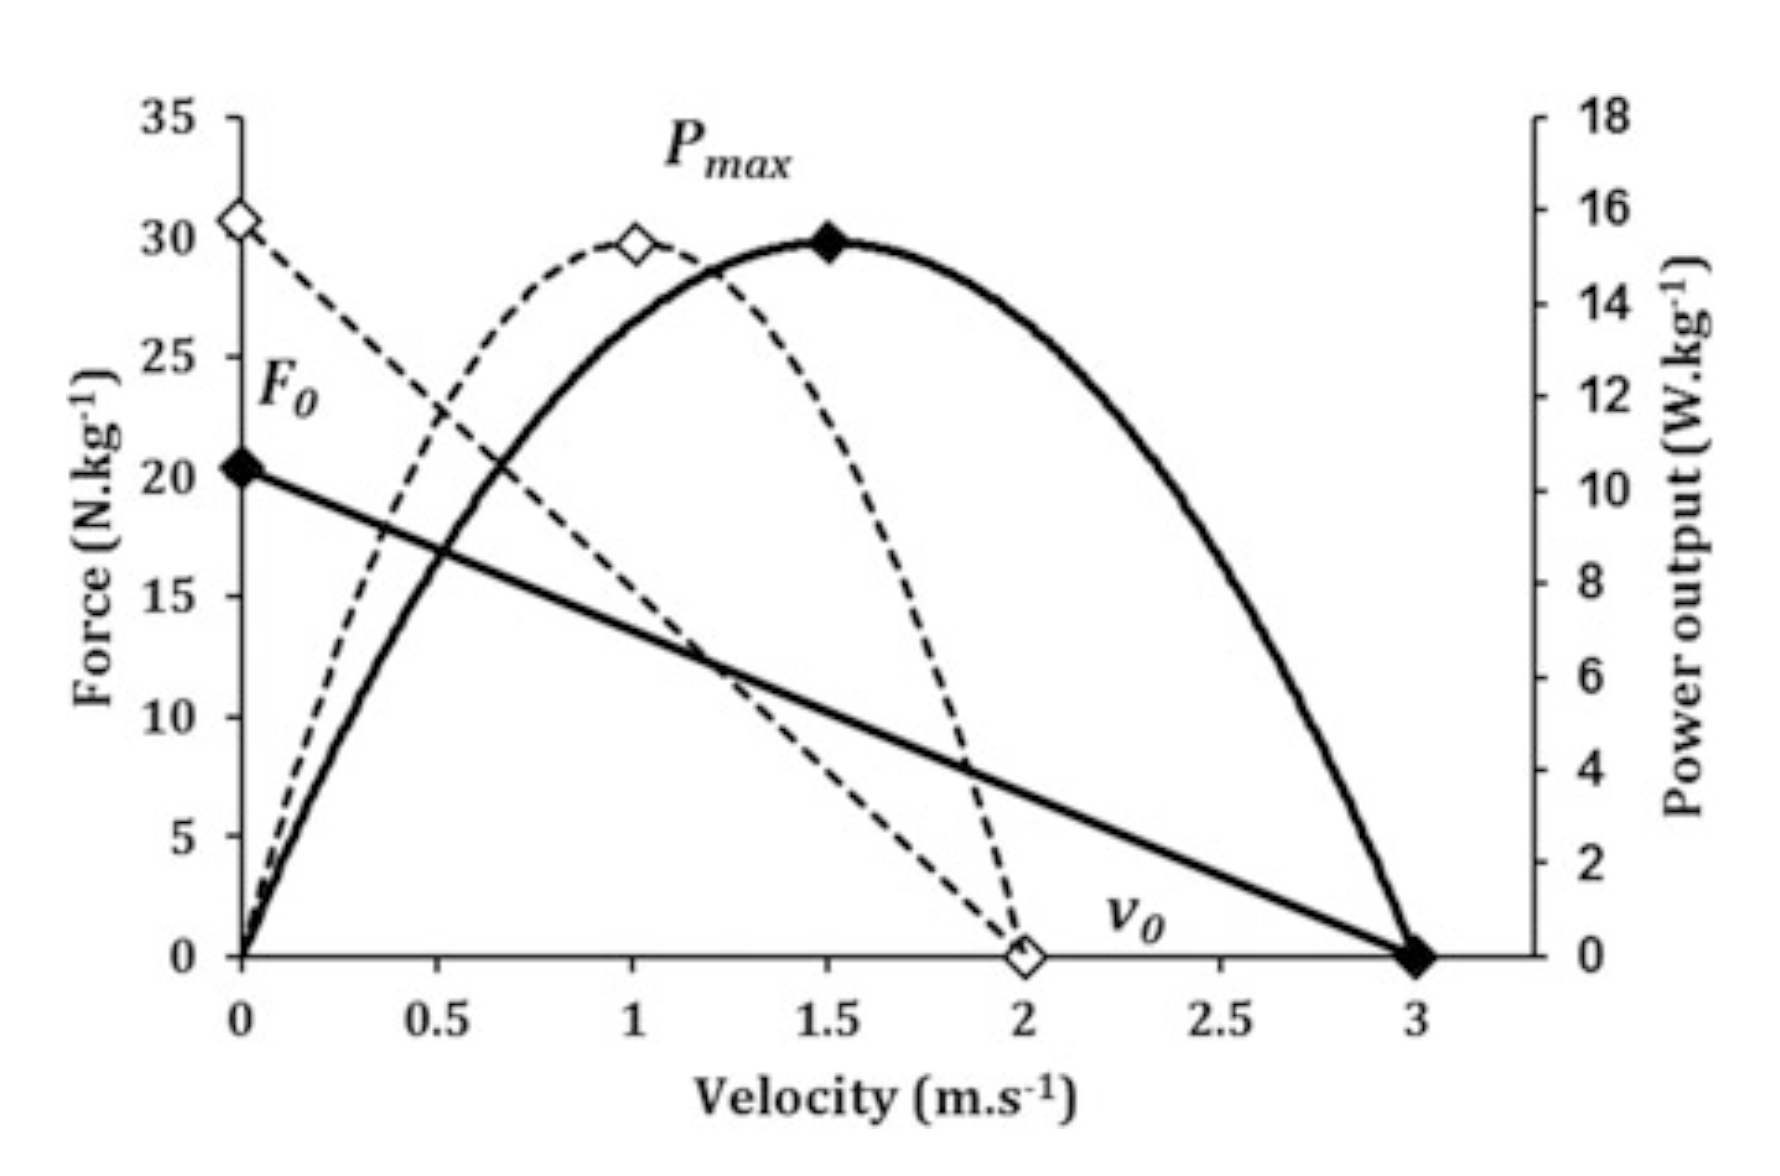
\includegraphics[width = 0.5\textwidth]{figure/Schermafbeelding 2022-11-21 om 16.08.08.png}
%     \caption{Force velocity curve and power}
%     \label{f_fv}
% \end{figure}
\subsection{Limitations and Future research}
\noindent\textbf{Tail length optimization leads to local maxima.} As seen in the results the tail length optimizations showed lower ollie height compared to the same optimizations with restricted tail length. This is per definition a local maximum because the solution space of the optimization with tail length optimized should contain the restricted tail length optimization solution. In real life a longer tail length would cause a higher energy dissipation due to more bending during impact \cite{stronge_impact_2000}. A plausible cause for these local maxima is that impact loss is of too little effect. When a human jumps, the order of magnitude of the amount of energy necessary to go up is in the order of $10^3$. The dissipation of energy during impact is in the order of $10^{-1}$. This means that the impact loss could be of so little effect to increasing ollie height that the solution space has become very flat. You can see that the model does capture the increase impact loss. When the tail length is optimized and the large tail length solution is found, there is an increase of 227\% compared to the base optimization. Maybe if the impact loss would be penalized more, optimal tail lengths will be found.
 
% Range of motion, balance, spacial skeletal constraints
\noindent\textbf{Lack of complexity in the kinematic constraints of the human controller.} Due to the simplification of a human as a mass point with two feet, kinematic constraints are highly simplified. In real life a penny board is difficult to ollie due to the fact that the operating area is really small. The feet would have to operate precise and powerful movements while balancing on a small surface. While the controller can easily do this, it does not represent reality completely. Also inertia of the human is neglected due to the simplification.

\noindent\textbf{Front wheel normal force.} In future research it is advised to implement a normal force acting on the front wheel during the preparation phase. The front foot had to counteract the rotation created by the back foot. In real life the front foot could have been on any location without causing a counter clockwise rotation due to the compensation of the normal force. Difficulties will be to find a phase switch cue for the optimizer. It might be possible to set a fixed time for the first phase to solve this.

\noindent\textbf{Possible that current solutions are not global optima, more optimal board shapes can be found.} The presented solution space is very large due to many possibilities in variables. In future research, many more geometries can be found which could help the skateboard community to understand the dynamics of the ollie. 

\noindent\textbf{Extra constraints should be implemented to the legs individually.} Now single leg behaviour can sometimes exceed human limitations. Due to a lack of data on single leg jump for one specific athlete together with the CMJ information the single leg behaviour is not yet fully bound by human limitations.


